\documentclass[USenglish,oneside,twocolumn]{article}

\usepackage[utf8]{inputenc}%(only for the pdftex engine)
%\RequirePackage[no-math]{fontspec}%(only for the luatex or the xetex engine)

% Do not change the template unless necessary
% Changing font sizes, margins or similar to make your project report appear longer
% than it is will lead to a failed exam.
\usepackage[big]{dgruyter_NEW}

\usepackage[backend=biber,natbib=false]{biblatex}
\addbibresource{references.bib}

% You can remove this include
\usepackage{blindtext}
  
\begin{document}
	
	

	\title{\huge SMART SECURITY DOOR LOCK SYSTEM: An IoT-Based Intelligent Access Control Solution}

\runningtitle{Smart Security Door Lock System}

\journalname{Internet of Things Projects}
\startpage{1}
	
 \section{Abstract}
  The Internet of Things (IoT) has changed conventional security systems, leading to more intelligent and dependable solutions. This research introduces the SMART SECURITY DOOR LOCK SYSTEM, a sophisticated IoT-powered access control solution. Utilizing the Pinecone BL602 microcontroller, the system combines motion detection, user verification, and servo motor-controlled door functions to provide secure, automated entry. A linked mobile app improves functionality, providing real-time alerts, access records, and remote management features. This system showcases the potential of IoT in transforming access control by tackling issues like unauthorized access and the drawbacks of physical keys. This pioneering security solution is scalable and focused on users, meeting the increasing need for smart infrastructure in contemporary homes and organizations.
\maketitle
	
	\section{Introduction}
    \label{sec:intro}
    In today’s world of smart devices and IoT technology, creating intelligent systems has become essential. Technology is changing the way we live, bringing more convenience, security, and ease into our daily lives. This project introduces the SMART SECURITY DOOR LOCK SYSTEM, a modern and advanced solution for access control and security. It solves problems with traditional lock-and-key systems, like losing keys or unauthorized duplication, while offering a secure and easy-to-use alternative. The system uses advanced hardware, including a Pinecone BL602 microcontroller, motion sensors, a reader module, and a servo motor. Together, these components automate door unlocking securely. It replaces physical keys with motion detection and digital authentication, making access safer and more convenient. A mobile app adds even more features, letting users manage access, view activity logs, and get alerts in real time. This makes it easy to monitor and control the system from anywhere, providing both security and convenience. The SMART SECURITY DOOR LOCK SYSTEM is flexible and can be used in homes, offices, and other spaces. Its design can also be upgraded in the future with features like biometric authentication or energy-saving options. This project shows how IoT can improve access control by making it smarter, more secure, and easier to use. It combines modern technology with practical design to create a system that meets today’s security needs and sets the foundation for future innovations.
	
    \section{Related Works}
	\label{sec:Related Works}

The development of smart door security systems is becoming more important, thanks to technologies such as RFID and microcontrollers. These innovations help solve problems with traditional locks, such as unauthorized access, lost keys, and lack of monitoring. Our project builds on these advancements to improve functionality and address their limitations. Traditional locks have been reliable for years, but come with problems such as lock picking, key duplication, and no real-time monitoring. Studies, such as those of this paper \cite{Shetty2020}, show that these locks don’t meet the security needs of modern homes and offices. Our project replaces physical keys with digital authentication to eliminate the risk of lost or duplicated keys and adds automated access control.

RFID technology is commonly used for secure access. For instance \cite{Ortiz2021}, designed an RFID-based door system that used a card to unlock doors. However, it lacked features like real-time notifications. Our system also uses RFID for security but goes further by adding IoT connectivity and sensors. This allows users to control the lock and receive notifications via a mobile app, which gives additional security details. Microcontrollers are essential for managing smart locks \cite{Ortiz2021}, used an Arduino microcontroller for RFID and motor control, while \cite{Edozie2020}, used Raspberry Pi for email alerts and better monitoring. These systems, however, often need more power. We chose the Pinecone BL602 microcontroller because it supports IoT features, consumes less power, and enables mobile app connectivity, making the system energy-efficient.

Mobile apps are crucial for smart locks, offering features like activity logs, real-time alerts, and easy control\cite{Edozie2020}, added an app for tracking door activity, and \cite{Tewari2021}, showed how apps make smart devices easier to use. Our app serves as the main control hub. Users can see the logs of whom all are opened the door and motion detection details like the person comes nears to the door motion, manage access, and receive alerts about unauthorized attempts in a simple, user-friendly way. IoT has revolutionized smart locks, allowing devices to connect to the internet for remote control and monitoring. Studies like those \cite{Edozie2020}, highlight the benefits of IoT-enabled systems, such as real-time alerts. Our project uses IoT to let users control and monitor the lock from anywhere. It also logs security events in the cloud, providing detailed insights for added convenience and peace of mind.

Despite their advantages, smart locks face challenges. RFID systems can experience signal problems near metal, and combining various hardware and software can be complex. To address these, we added proximity sensors to improve reliability and used modular hardware for easier integration. The Pinecone BL602 microcontroller \cite{PINE64}, also ensures low power use, allowing the system to run efficiently, even on batteries. Our project gives security with authentication, by combining RFID, motion sensors, and wifi connection to ensure only authorized users gain access and others cannot get the access. Motion sensors also detect intrusions and send alerts, providing an extra layer of safety. Our SMART SECURITY DOOR LOCK SYSTEM improves on traditional locks and earlier smart systems by combining IoT, RFID, and mobile app functionality. It offers a secure, energy-efficient, and easy-to-use solution for protecting homes, offices, and other spaces.

    

\section{System Design and Implementation}
\label{sec:System Design and Implementation}
The Smart Security Door Lock System is designed to be simple, affordable, and easy to use. It has two main parts: the hardware, which includes all the physical components like the RFID reader, motion sensor, servo motor, Wi-Fi module, and Pinecone microcontroller; and the software, which is the mobile app that makes everything work seamlessly together. We have focused on creating a user-friendly system that doesn’t cost too much, making it a great choice for improving home or office security.

(Fig1) The figure shows the circuit we developed. By looking at the diagram, we can see how the components are connected. The RFID reader (EM18)\cite{RFIDReaderEM18}, is the key part of the system where everything starts. When the user taps their RFID card on the reader, the module reads the card and checks if the person is authorized. If the card is valid, the RFID reader sends a signal to the Pinecone microcontroller.

The Pinecone microcontroller is like the brain of the system. Once it gets the signal from the RFID reader, it checks the user’s credentials. If everything is correct, the Pinecone sends a signal to the servo motor, which then unlocks the door by rotating. This process makes sure only authorized users can access the door.

To make the system even smarter, a motion sensor is added. This sensor detects any movement near the door, which can help identify if someone unauthorized is trying to enter. If unusual motion is detected, the system sends an alert through the mobile app, letting the user know what’s happening in real-time.

The Wi-Fi module connects the Pinecone microcontroller to the mobile app. This connection allows the user to monitor the door, get alerts, and manage access permissions from anywhere. The app, built using Android Studio, acts as the system’s control panel. It shows who accessed the door, when it was accessed, and even sends notifications about unauthorized attempts or motion detection.  
\begin{figure}[h!]
    \centering
    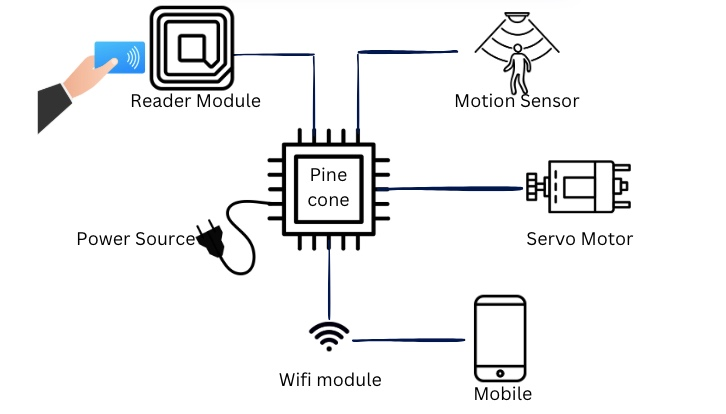
\includegraphics[width=0.5\textwidth]{architecture.jpeg}
    \caption{System Architecture of the SMART SECURITY DOOR LOCK SYSTEM with Servo Motor}
    \label{fig:system_architecture}
\end{figure}


\begin{figure}[h!]
    \centering
    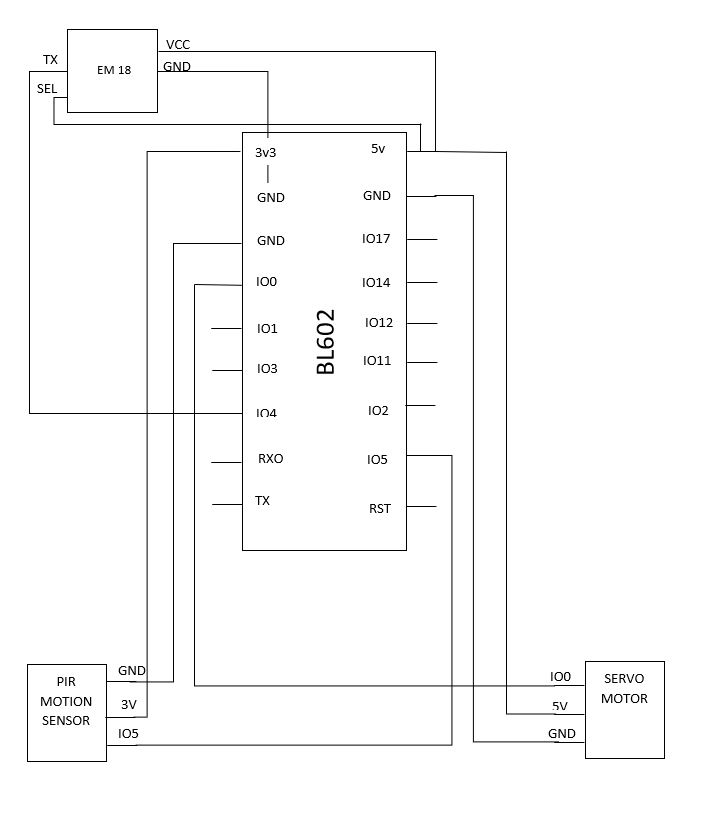
\includegraphics[width=0.5\textwidth]{pin diagram.JPG}
    \caption{Circuit diagram of the of the SMART SECURITY DOOR LOCK SYSTEM }
    \label{fig:pin diagram}
\end{figure}

\section{Implementation}
\label{sec:Implementation}

\subsection{Hardware Integration}

The hardware integration for the SMART SECURITY DOOR LOCK SYSTEM involves connecting multiple components to the Pinecone BL602 microcontroller, ensuring synchronized operation for secure and efficient functionality. The system integrates an EM-18 RFID reader, a servo motor, a PIR motion sensor, and a Wi-Fi module, all connected properly as per the provided pin diagram to enable robust communication and control. The EM-18 RFID reader is responsible for scanning RFID tags. It is connected to the microcontroller using the UART interface, with the RFID TX pin linked to the RX pin of the microcontroller (GPIO4). The reader operates at a baud rate of 9600 bps, configured using the firmware to ensure accurate data transmission. The RFID tag values are hardcoded into the microcontroller's memory, and when a tag is scanned, its value is matched against these stored credentials.The code \texttt{\#define VALID\_RFID "3800B7DCFCAF"} hardcodes the RFID tag value \texttt{"3800B7DCFCAF"} into the code, which is used for comparison to verify if a scanned RFID tag matches the predefined valid tag.
 Upon successful authentication, the microcontroller sends a signal to the servo motor\cite{MG996RServoMotor} to unlock the door. The TIMEOUT\_MS macro defines a timeout period of 1000 milliseconds (1 second), which is used in the read\_rfid\_tag() function to check if an RFID tag has been received within this time. If the timeout is exceeded, the function processes the tag, null-terminates it, and performs the necessary actions like tag verification.

\begin{figure}[h!]
    \centering
    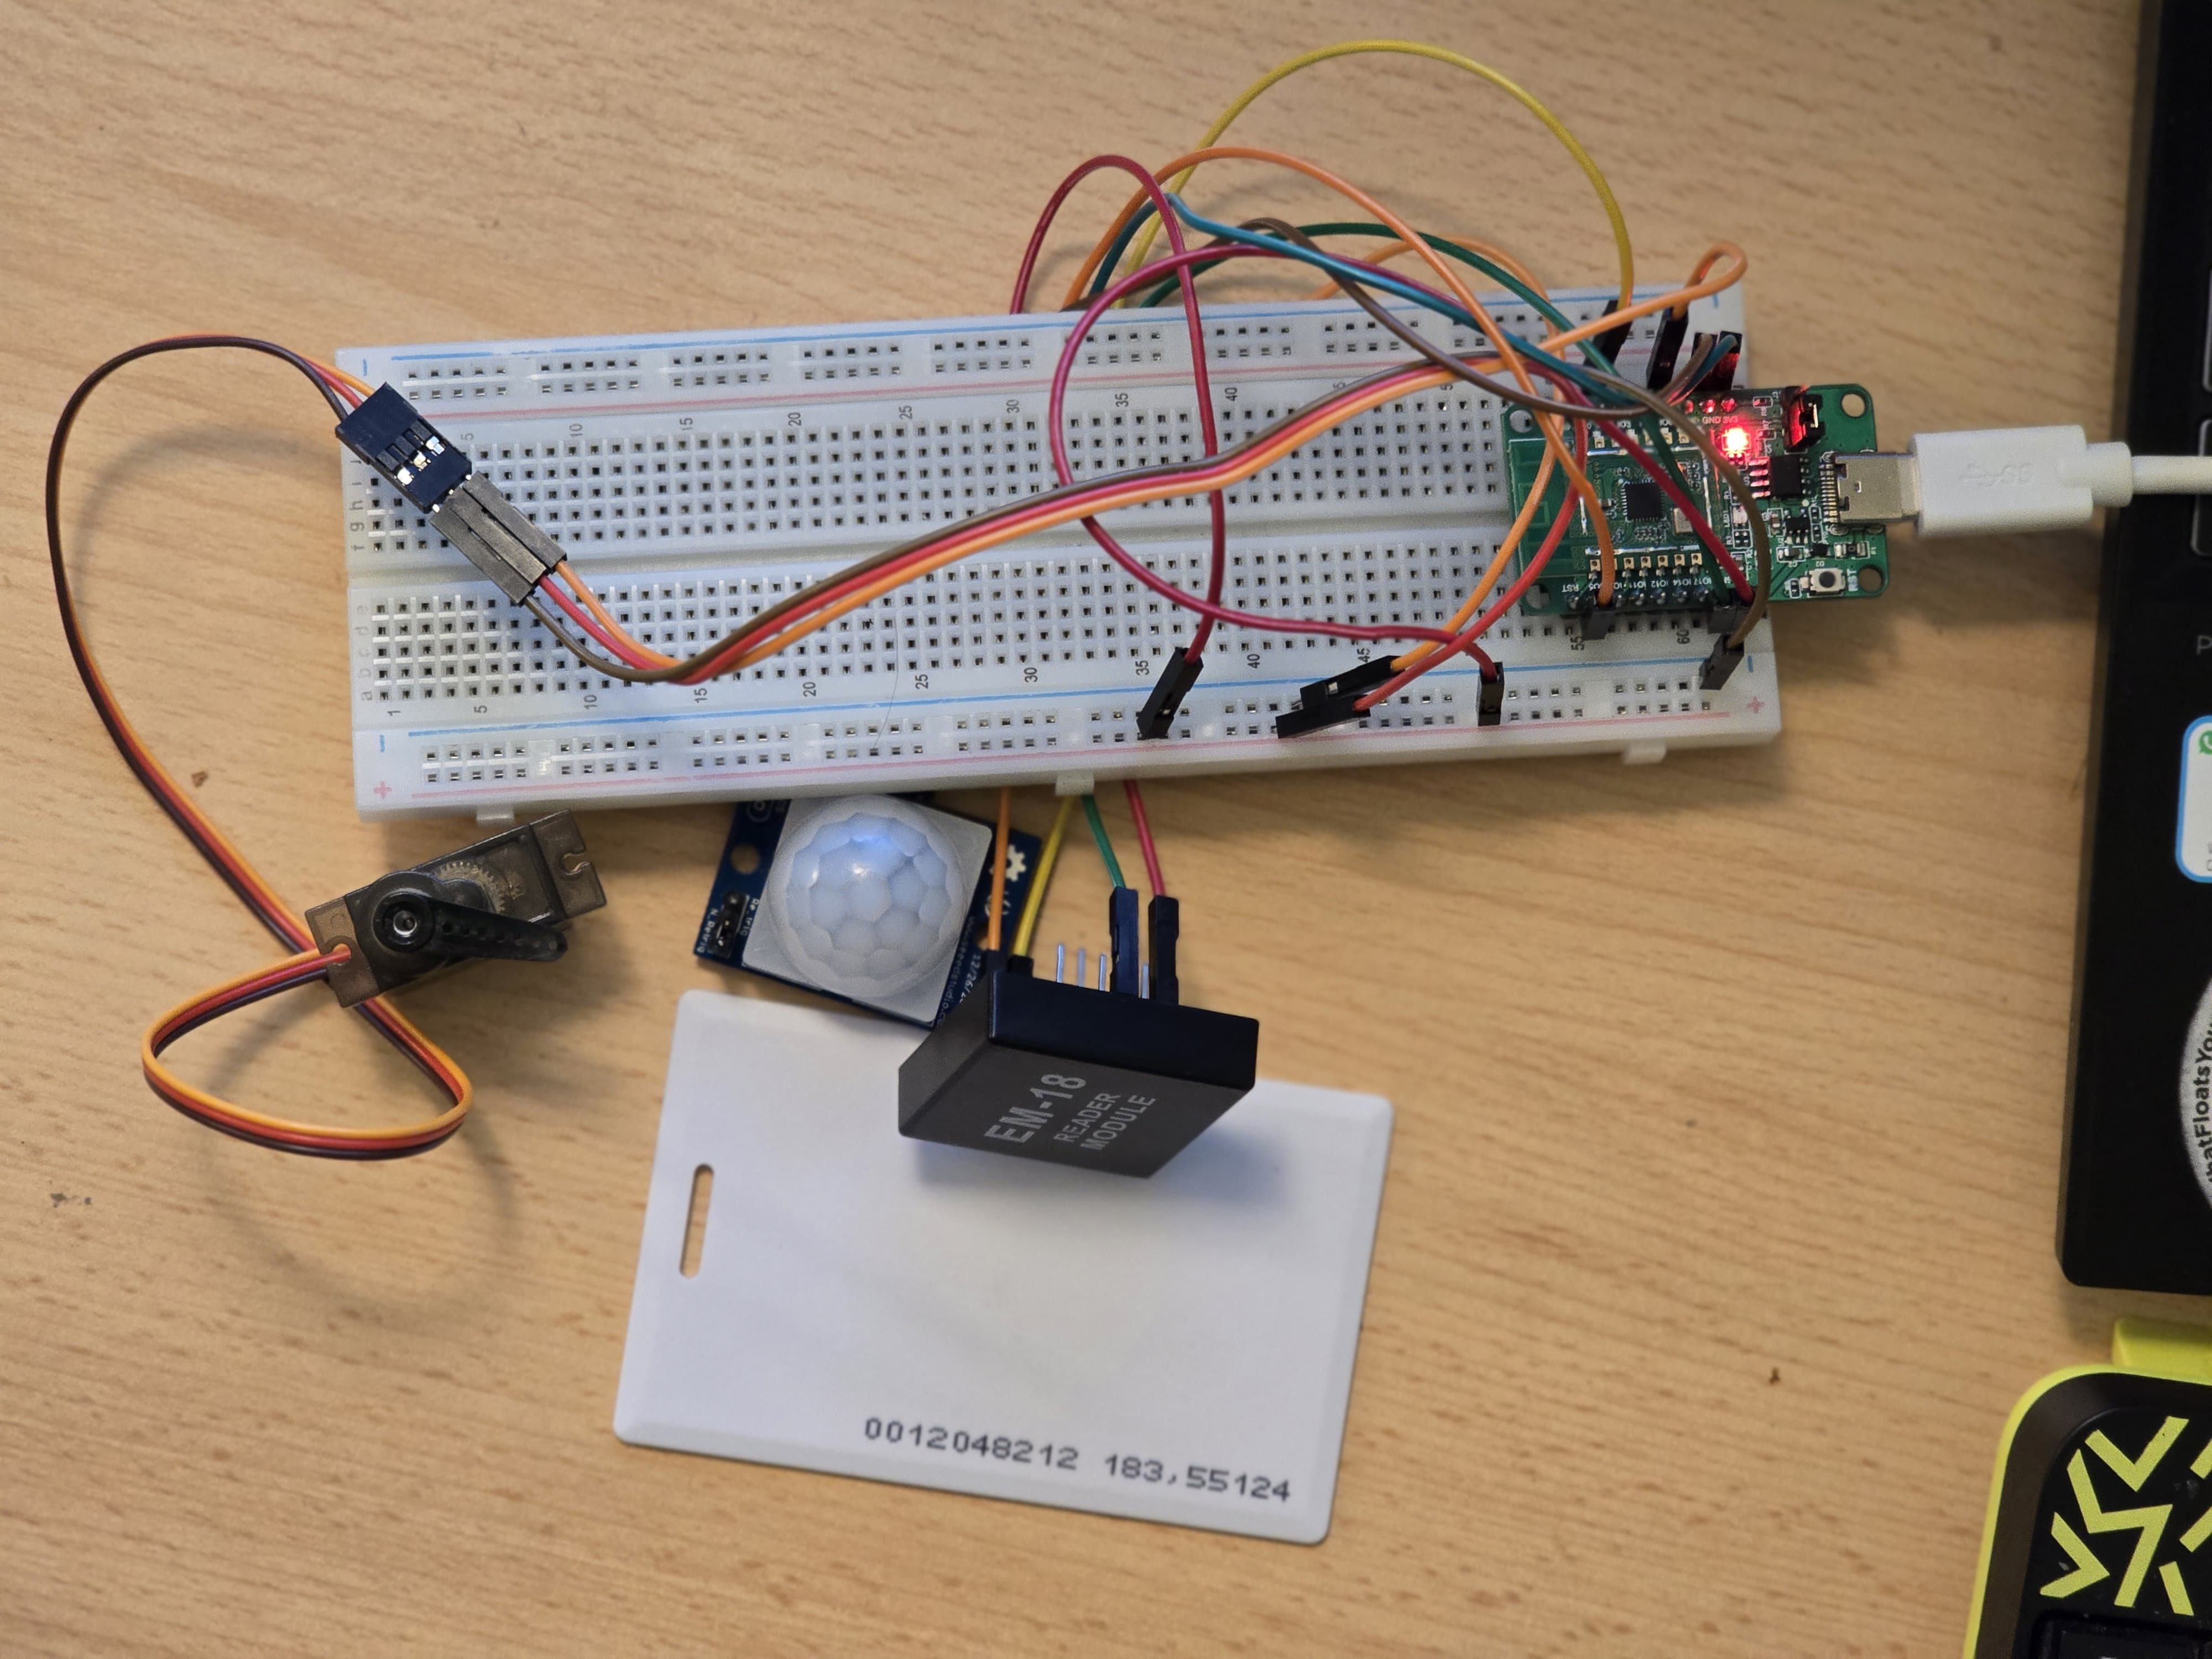
\includegraphics[width=0.5\textwidth]{hardware_connections.jpeg}
    \caption{Hardware Connections}
    \label{fig:hardware_connections}
\end{figure}

The servo motor, responsible for physical door movement, is connected to the microcontroller’s IO5 pin. When triggered, the motor rotates to open the door and remains in this position for 20 seconds before returning to its initial state to secure the door. The 5V power supply to the motor ensures smooth and stable operation, while its connection to the microcontroller guarantees precise control. The PIR motion sensor is another critical component. It has a specific role that we planned in the early stages of our project, which is to continuously monitor the area near the door and send activity signals to the microcontroller. If motion is detected, it triggers a log update, alerts the user via the mobile app, and makes the LED blink red to indicate detected motion. Conversely, if no motion is detected, the LED remains off, providing a clear visual indicator of the system's status. The sensor is powered by a 3V supply, optimizing power efficiency while maintaining sensitivity.

The integration of the Wi-Fi module further enhances the system by enabling wireless communication. It connects the Pinecone BL602 microcontroller to the mobile app, facilitating remote monitoring and control. The Wi-Fi module is initialized in the firmware to establish a seamless network connection. This enables users to manage access, receive real-time notifications, and monitor logs remotely, adding convenience and security. The pin connections ensure robust and modular integration, allowing for easy troubleshooting and future enhancements. The 3.3V and 5V power supply pins are used judiciously to power the components without overloading the microcontroller. Ground (GND) pins are appropriately shared to maintain a common reference, ensuring signal integrity across all connections.

We wanted to add some problems which we faced on here they are. The first challenge was working with the EM-18 sensor. The EM-18 has a different baud rate (9600 bps), which required switching the baud rate from the default 2 Mbps to 9600 bps. This required setting up multiple UARTs, which was quite challenging. Additionally, the EM-18 sensor lacks an RX pin, only having a TX pin (RX - Receiver, TX - Transmitter). This meant that the TX pin of the EM-18 had to be connected to the RX pin of the Pinecone and vice versa, which posed setup issues. Understanding how the TX and RX pins work also took some time. Another difficulty was the selection pin of the EM-18, which needs to be connected to the same voltage as the VCC. Understanding this requirement and configuring the code to accommodate it led to significant troubleshooting and challenges. At the end we found the solution and we made it to work.

Our prototype which we planned to make it with help of 3D printing and small house in which we will be keeping reader module near to the door and the door is attached with a shaft with the servo motor so the door will open without trouble and pinecone will be in the center part of our model house the motion sensor will be placed next to the door. 


\subsection{Software Integration:}The Smart Security Door Lock System uses software to make the system easy, secure, and convenient for users. The mobile app, built using Android Studio using the Java Programming language, connects with the hardware through a Wi-Fi module. For the app to work, it must be on the same Wi-Fi network as the hardware. This connection lets users control and monitor the system in real time. However, creating this system was not easy and required a lot of problem-solving.

We initially faced challenges integrating the motion sensor with the Pinecone BL602 microcontroller, as it either gave false alerts or failed to detect motion accurately, but adjustments ensured reliable real-time updates. Additionally, while building our Android app, we faced an issue where the WebView failed to load web content, which we resolved by adding the INTERNET permission in the AndroidManifest.xml. These challenges taught us valuable lessons and improved the overall system.

The software works through the mobile app, which has four main features. Each feature connects to a specific URL, called an endpoint. These features make it easy for users to manage the system:

\begin{itemize}
    \item To  see motion detection :\\
    \texttt{http://192.168.169.1/motion.html}
\end{itemize}

The mobile  app uses the above url to check for motion near the door. If someone comes close, the motion sensor detects it and updates the app in real time. This helps users know if someone is at their door, whether it’s a visitor or an unauthorized person.

Over time, the motion sensor creates a log of all detected movements. If too many logs build up, it can clutter the system and makes problem in the performance. So, we found a solution to fix this, 

The below endpoint feature allows users to delete old logs with one tap, keeping the system clean and organized.
\begin{itemize}
    \item To clear motion logs:\\
    \texttt{http://192.168.169.1/clearmotion.html}
\end{itemize}

This below endpoint feature allows users to see who are all logged in using RFID Tag to open the door with their details.
\begin{itemize}
    \item To view logged details:\\
    \texttt{http://192.168.169.1/doorstatus.html}
\end{itemize}


The motion detection feature is especially important because it adds an extra layer of security. Whenever someone comes near the door, the app provides a real-time update. This ensures users are always aware of what’s happening around their home or office, even when they are not there. Building the software was a learning experience. Early on, we faced many issues, including unreliable motion detection, problems connecting the app and hardware to the same Wi-Fi, and creating an app interface that was easy to use. It took a lot of testing and refining to solve these problems. We decided to focus on making RFID and motion detection work perfectly rather than adding features that the hardware couldn’t support. This decision helped us create a simpler and more reliable system.

\begin{figure}[h!]
    \centering
    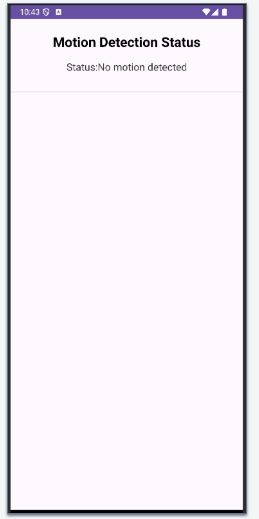
\includegraphics[width=0.15\textwidth]{no motion.JPG}
    \caption{ No motion detected}
    \label{fig:no motion}
\end{figure}


\begin{figure}[h!]
    \centering
    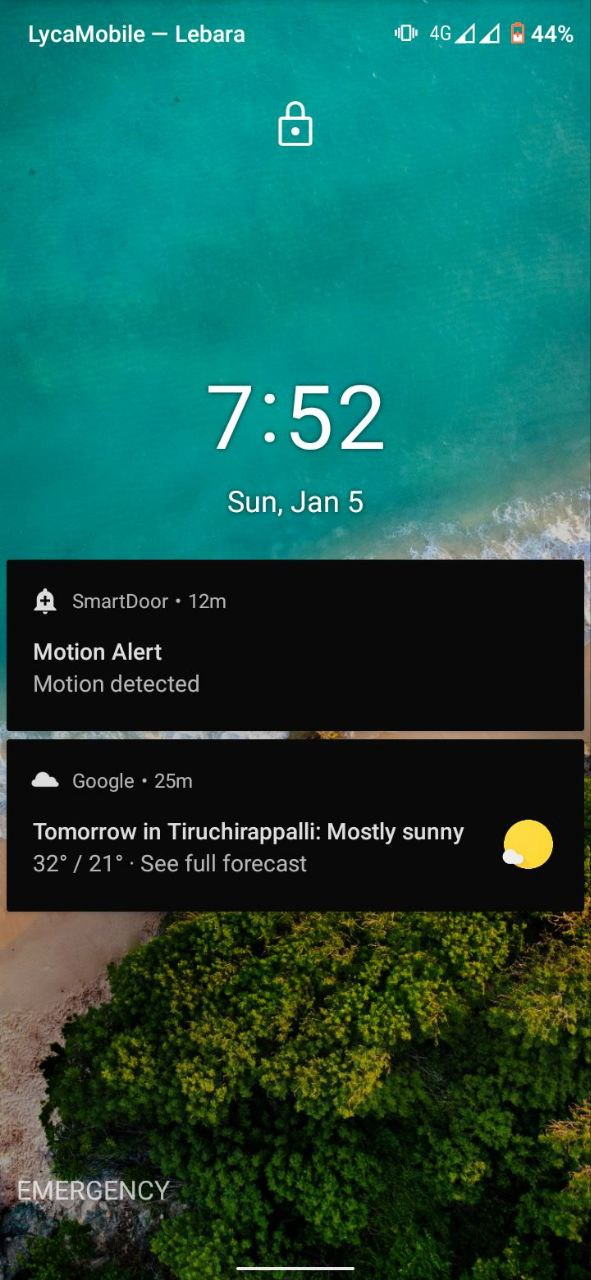
\includegraphics[width=0.15\textwidth]{motion notification.jpg}
    \caption{ Motion alert}
    \label{fig:motion alert}
\end{figure}

The result is a mobile app that brings all these features together in one place. Users can easily manage their system with just a few taps on their phone. The app makes the Smart Security Door Lock System more secure and convenient, giving users peace of mind. It turns a traditional lock into a smart solution that works for homes, offices, and other spaces. By combining IoT technology, real-time monitoring, and a user-friendly app, this system is a big step forward in modern security. It is simple to use, reliable, and effective,making it a valuable tool for keeping spaces safe and secure.

\section{Evaluation}
\label{sec:Evaluation}
During the evaluation face of our Smart Security Door Lock System project, we faced several challenges and made significant progress by adapting our approach. Initially, we aimed to use the R307S fingerprint sensor for opening the door, as it offered a highly secure and modern solution. However, integrating this sensor proved to be very difficult due to hardware limitations and processing requirements. Despite more effort to resolve these issues, we were unable to make the fingerprint sensor function reliably within the scope of our system. So, we changed our plan to work on an alternative solution which is to use the RFID-based solution using the EM18 sensor, which proved to be a lightweight and efficient alternative.

The EM18 RFID sensor emerged as a practical choice at this time because it is less demanding in terms of processing power and still provides a secure and hygienic access control option. Because nowadays so many viruses are spreading though physical contact so we wanted to avoid physical contact. Bascially, The sensor can read RFID cards within a maximum range of 3 inches, which enhances security by requiring close proximity while also being convenient and touchless. This touchless feature is especially valuable for maintaining hygiene in shared or public spaces, as users do not need to make direct contact with the sensor. 

To support this hardware, we developed APIs for managing the key functionalities of the system.
Motion Detection API to monitor real-time activity near the door, ensuring that any movement is logged for security purposes. We implemented Clearing Motion Logs, our next API, deletes old motion logs to keep the system organized and ensure that excessive logs do not degrade performance or clutter the log history, so we wanted to keep log history clean.
RFID Access Logs API that tracks and stores the history of users who accessed the system, allowing easy review of who entered and when. We wanted to give additional security,  with this they can see who are all inside the house. RFID Access Logs can be cleared, we also have an API for this which helps use to clean the logs.

In addition to the RFID system, the motion sensor performed exceptionally well, accurately detecting movement around the door and triggering alerts as needed. This added another layer of security by detecting potential intrusions or unauthorized access attempts. The servo motor, powered by a 5V supply, reliably managed the locking and unlocking mechanism, ensuring smooth operation throughout our testing. We Have a special feature if some one lost their access card means we can remove the card access so no one can access the door with the lost card. As a result, the security is high and people don't have to worry about their lost card. 

Finally, our project is functional with all the added sensors and with the software we worked and delivered our best to maximize our project performance.
	
	\section{Conclusion}
\label{sec:Conclusion}

Bringing our Smart Security Door Lock System to life has been a journey full of learning and adjustments. At first, we imagined a system packed with advanced features that would combine security, convenience, and modern technology. We wanted it to be more than just a door lock  it had to be a smarter, easier way to control access, stop unauthorized entry, and improve security for homes or offices. While building the system, we faced some challenges. Some parts didn’t work as expected, and it was difficult to put all our ideas together into one smooth design. To solve these issues, we simplified our approach and focused on making the system efficient and practical. Using the Pinecone microcontroller as the core, along with key components like the RFID reader, motion sensor, Wi-Fi module, and mobile app, we created a system that works effectively.

Although we couldn’t include every idea we started with, what we have built is strong, reliable, and highly functional. Our Smart Security Door Lock System isn’t just a lock it’s a complete solution designed to make security easier and more convenient. It uses motion sensors to detect activity, an RFID reader for secure access, and a mobile app that acts as a control panel for users. This makes managing security simple while keeping homes and offices safe. The idea of a smart security system combines  hardware, effective control features, and user friendly mobile app. Our system is an innovative step forward in IoT technology. It not only achieves the goals we set but also goes beyond our expectations in terms of usefulness and flexibility. By replacing traditional locks with modern technology, the Smart Security Door Lock System offers valuable benefits and a glimpse into the future of smart home security. Our system is ready to improve lives by offering a perfect mix of safety, convenience, and innovation. 


	% Show cited references
	\printbibliography[title={References}]
\end{document}
